
% !TeX root = raytracing/slides/main.tex
% raytracing_preamble.tex
% Common styling for Ray Tracing presentation

\documentclass[10pt]{beamer}
\usetheme{metropolis}
\usefonttheme{professionalfonts}

% --- Color Definitions ---
\definecolor{PrimaryColor}{RGB}{33,52,72}         % Deep navy
\definecolor{SecondaryColor}{RGB}{84,119,146}     % Desaturated blue-gray
\definecolor{AccentColor}{RGB}{100, 156, 165}       % Soft steel blue

\definecolor{BackgroundColor}{RGB}{245,247,250}   % Very light cool gray/blue-tinted white
\definecolor{TextColor}{RGB}{40,55,70}            % Darker, cool-toned charcoal (slightly less saturated)
\definecolor{LightGray}{RGB}{220,225,230}         % Soft, cool light gray
\definecolor{DarkGray}{RGB}{70,90,105}            % Cool-toned dark gray (coherent with Primary/Secondary)

\definecolor{RayColor}{RGB}{230,150,80}           % Muted warm orange (less saturated than pure orange)
\definecolor{ObjectColor}{RGB}{128,101,160}       % Muted violet (adjusted purple to match cool palette)
\definecolor{LightColor}{RGB}{235,200,100}        % Soft golden yellow (to complement cool blues)

% --- Theme Customization ---
\setbeamercolor{background canvas}{bg=BackgroundColor}
\setbeamercolor{normal text}{fg=TextColor}
\setbeamercolor{frametitle}{bg=PrimaryColor, fg=white}
\setbeamercolor{section in toc}{fg=PrimaryColor}
\setbeamercolor{block title}{bg=PrimaryColor!80, fg=white}
\setbeamercolor{block body}{bg=PrimaryColor!10}
\setbeamercolor{alerted text}{fg=AccentColor}
\setbeamercolor{itemize item}{fg=PrimaryColor}
\setbeamercolor{itemize subitem}{fg=SecondaryColor}
\setbeamerfont{frametitle}{size=\large,series=\bfseries}

% --- Packages ---
\usepackage[utf8]{inputenc}
\usepackage{url}
\usepackage{booktabs}
\usepackage{amsmath, amssymb}
\usepackage{fontawesome5}
\usepackage{pifont}
\usepackage[most]{tcolorbox}
\tcbuselibrary{skins}
\usepackage{colortbl}
\usepackage{array}
\usepackage{tikz}
\usepackage{graphicx}
\usetikzlibrary{shapes.callouts, positioning, arrows.meta, shapes.geometric, shadows, calc, patterns, 3d, backgrounds, shadings}
\usepackage{adjustbox}
\usepackage{ragged2e}
\usepackage{pgfplots}
\usepackage{graphicx}
\usepackage{caption}
\usepackage{minted}
\pgfplotsset{compat=1.18}

% --- Custom Commands ---
\newcommand{\cmark}{\textcolor{SecondaryColor}{\ding{51}}}
\newcommand{\xmark}{\textcolor{AccentColor}{\ding{55}}}
\newcommand{\highlight}[1]{\textcolor{PrimaryColor}{\textbf{#1}}}
\newcommand{\raycolor}[1]{\textcolor{RayColor}{\textbf{#1}}}
\newcommand{\objectcolor}[1]{\textcolor{ObjectColor}{\textbf{#1}}}

% --- TikZ styles for ray tracing visualizations ---
\tikzstyle{process} = [rectangle, rounded corners=3mm, minimum width=2cm, minimum height=0.8cm, text centered, draw=PrimaryColor, thick, fill=PrimaryColor!15, drop shadow]
\tikzstyle{arrow} = [thick, PrimaryColor, ->, >=stealth]
\tikzstyle{ray} = [thick, RayColor, ->, >=stealth]
\tikzstyle{lightray} = [thick, LightColor, ->, >=stealth]
\tikzstyle{reflectray} = [thick, SecondaryColor, ->, >=stealth]
\tikzstyle{refractray} = [thick, AccentColor, ->, >=stealth]
\tikzstyle{shadowray} = [thick, DarkGray, ->, >=stealth, dashed]

% --- 3D object styles ---
\tikzstyle{sphere} = [circle, minimum size=1.5cm, draw=ObjectColor, thick, fill=ObjectColor!20, drop shadow]
\tikzstyle{plane} = [rectangle, minimum width=3cm, minimum height=0.2cm, draw=ObjectColor, thick, fill=ObjectColor!20]
\tikzstyle{triangle} = [regular polygon, regular polygon sides=3, minimum size=1.5cm, draw=ObjectColor, thick, fill=ObjectColor!20]

% --- Eye/Camera styles ---
\tikzstyle{eye} = [circle, minimum size=0.8cm, draw=PrimaryColor, thick, fill=PrimaryColor!30]
\tikzstyle{pixel} = [rectangle, minimum size=0.2cm, draw=AccentColor, fill=AccentColor!30]

% --- Text box styles ---
\tikzstyle{conceptbox} = [rectangle, rounded corners, fill=PrimaryColor!10, draw=PrimaryColor, thick, text width=0.8\textwidth, inner sep=8pt]
\tikzstyle{formulabox} = [rectangle, rounded corners, fill=SecondaryColor!10, draw=SecondaryColor, thick, inner sep=6pt]

% --- Custom environments ---
\newtcolorbox{raybox}[1]{
  colback=RayColor!10,
  colframe=RayColor,
  title=#1,
  fonttitle=\bfseries,
  sharp corners
}

\newtcolorbox{conceptbox}[1]{
  colback=PrimaryColor!10,
  colframe=PrimaryColor,
  title=#1,
  fonttitle=\bfseries,
  rounded corners
}

\newtcolorbox{mathbox}[1]{
  colback=SecondaryColor!10,
  colframe=SecondaryColor,
  title=#1,
  fonttitle=\bfseries,
  rounded corners
}

\newenvironment{timeline}{%
  \begin{tikzpicture}[scale=0.8]
    \coordinate (start) at (0,0);
    \newcounter{timelineitem}
    \setcounter{timelineitem}{0}
  }{%
  \end{tikzpicture}
}

\newcommand{\timelineitem}[4]{%
  \stepcounter{timelineitem}%
  % Name of this item’s node
  \edef\thisID{time\thetimelineitem}%
  \ifnum\value{timelineitem}=1
  % First item: anchor at (start)
  \node[rectangle, draw, fill=PrimaryColor!20,
  text width=1.5cm, minimum height=0.8cm, align=center]
  (\thisID) at (start) {\textbf{#2}};
  \else
  % Later items: below=#1 of previous time node
  \pgfmathtruncatemacro\prev{\value{timelineitem}-1}%
  \node[rectangle, draw, fill=PrimaryColor!20,
    text width=1.5cm, minimum height=0.8cm, align=center,
  below=#1 of time\prev]
  (\thisID) {\textbf{#2}};
  \fi
  % Description always to the right of this time node
  \node[rectangle, draw, fill=SecondaryColor!10,
    text width=4cm, minimum height=0.8cm,
  align=left, right=0.3cm of \thisID]
  (desc\thetimelineitem) {\textbf{#3}\\#4};
  % Draw arrow back to previous if not the first
  \ifnum\value{timelineitem}>1
  \draw[->, thick, PrimaryColor]
  (time\prev.south) -- (\thisID.north);
  \fi
}

\tikzset{
  camera/.style={fill=PrimaryColor!60, draw=PrimaryColor!80, rectangle, minimum size=8pt},
  image plane/.style={fill=AccentColor!10, draw=AccentColor!50, opacity=0.8},
  pixel/.style={fill=AccentColor!60, thick},
  primary ray/.style={->, very thick, red!90},
  object/.style={fill=ObjectColor!60, draw=ObjectColor!80, circle, minimum size=12pt},
  fovangle/.style={<->, thick, PrimaryColor, dashed}
}

\tikzset{
  lens/.style={thick, PrimaryColor, line width=3pt},
  focal plane/.style={thick, AccentColor},
  object ray/.style={->, thick, ObjectColor},
  image ray/.style={->, thick, SecondaryColor},
  optical axis/.style={dashed, gray}
}

\newcommand{\lens}[3]{%
  \begingroup
  % half‐dimensions
  \pgfmathsetlengthmacro{\a}{#2}%
  \pgfmathsetlengthmacro{\b}{#3}%
  \pgfmathsetlengthmacro{\c}{#3/2}%
  \begin{scope}[shift={#1}]
    \draw[line join=round, fill=blue!15]
    (0,-{\c})
    arc(-30:30:{\a} and {\b})
    arc(150:210:{\a} and {\b})
    ;
  \end{scope}
  \endgroup
}

\title{Fractals}
\subtitle{Infinite Details from Simple Rules}
\author{\large Ashrafur Rahman}
\date{\small Adjunct Lecturer}
\institute{Department of Computer Science and Engineering\\ Bangladesh University of Engineering and Technology (BUET)}

\begin{document}

\begin{frame}
  \titlepage
\end{frame}

\section{Definition}

\begin{frame}{What are Fractals?}
  \begin{conceptbox}{Definition}
    A \highlight{fractal} is a geometric shape containing detailed structure at arbitrarily small scales,
    usually having a \highlight{fractal dimension} strictly exceeding the \highlight{topological dimension}.
  \end{conceptbox}

  \vspace{0.1cm}

  \textbf{Key Characteristics:}
  \begin{itemize}
    \item \highlight{Scale invariance}: Details at every level of magnification
    \item \highlight{Fractal dimension}: More than the \textit{conventional} dimension
    \item \highlight{Infinite complexity}: Generated by simple, recursive rules
      \begin{itemize}
        \item Like the infinite complexities of nature
      \end{itemize}
  \end{itemize}

  \vspace{0.1cm}

  \pause
  \begin{center}
    \tikz[scale=0.8]{
      \node[conceptbox, text width=0.7\textwidth] {
        \centering
        \textit{"Clouds are not spheres, mountains are not cones, coastlines are not circles..."} \\
        \textbf{— Benoit Mandelbrot}
      };
    }
  \end{center}
\end{frame}

\section{Some Fractals}

\begin{frame}{The Sierpinski Triangle}
  \begin{columns}
    \begin{column}{0.6\textwidth}
      \small
      \only<1-6>{
        Let's construct the Sierpinski Triangle:
        \begin{conceptbox}{Construction Process}
          \footnotesize
          \begin{enumerate}
            \item Start with an equilateral triangle
            \item<2-> Remove the central triangle (triangle connecting midpoints of the sides)
            \item<3-> Repeat for each triangle
            \item<4-> After infinite iterations, we get the Sierpinski Triangle
          \end{enumerate}
        \end{conceptbox}
      }

      \only<7-10>{
        Now let's find the area of triangle(s):
        \begin{mathbox}{Area Calculation}
          \footnotesize
          \begin{align*}
            \only<7->{
              A_0 &= \frac{1}{2}\cdot \sin(60^\circ) \cdot a^2 = \frac{\sqrt{3}}{4} a^2 \\
            }
            \only<8>{
              A_1 &= A_0 - \frac{1}{2}\cdot \sin(60^\circ) \cdot \left(\frac{a}{2}\right)^2 \\
              &= A_0 - \frac{\sqrt{3}}{16} a^2 = A_0 - \frac{1}{4} A_0 \\
              &= \frac{3}{4} A_0
            }
            \only<9->{
              A_1  &= \left(1-\frac{1}{4}\right) A_0 =  \frac{3}{4} A_0 \\
              A_2 &= \left(1-\frac{1}{4}\right) A_1 = \left(\frac{3}{4}\right)^2 A_0 \\
            }
            \only<10->{
              \hdots \\
              A_n &= \left(1-\frac{1}{4}\right)^n A_0 = \left(\frac{3}{4}\right)^n A_0 \\
              \lim_{n \to \infty} A_n &= 0
            }
          \end{align*}

        \end{mathbox}
        \only<8-9>{
          We cut out one fourth of the area at each step. So, naturally area is reduced by $\frac{3}{4}$ at each step.
        }
        \only<10->{
          \highlight{The area of the Sierpinski Triangle is zero even though it is a 2D shape.}
        }

      }

      \only<11-14>{
        Now let's find the perimeter:
        \begin{mathbox}{Perimeter Calculation}
          \footnotesize
          \begin{align*}
            \only<11->{
              P_0 &= 3a \\
            }
            \only<12->{
              P_1 &= P_0 + 3\cdot\frac{a}{2} = \frac{9}{2} a = \frac{3}{2} P_0 \\
            }
            \only<13->{
              P_2 &= P_1 + 3\cdot3\cdot\frac{a}{4} = P_1 + \frac{1}{2} P_1 = \frac{3}{2} P_1 \\
            }
            \only<14->{
              \hdots \\
              P_n &= \frac{3}{2} P_{n-1} = \left(\frac{3}{2}\right)^n P_0 \\
              \lim_{n \to \infty} P_n &= \infty
            }
          \end{align*}
        \end{mathbox}
        \only<12-13>{
          We add half of the previous perimeter at each step.
          This is because we add the same number of triangles as the last step,
          but each triangle is half the size of the previous one.

          As a result, the perimeter grows by a factor of $\frac{3}{2}$ at each step.
        }
        \only<14->{
          \highlight{The Sierpinski Triangle has infinite perimeter but zero area.}
        }
      }

    \end{column}
    \begin{column}{0.4\textwidth}
      \begin{center}
        \begin{center}
          \begin{figure}
            \foreach \t/\i in {1/0,2/1,3/2,4/3,5/4,6/5} {
              \only<\t>{
                \includegraphics[width=\textwidth]{images/sierpinski/\i.png}
                \caption*{Iteration \i}
              }
            }
            \foreach \t/\i in {7/0, 8/1, 9/2, 10/3} {
              \only<\t>{
                \includegraphics[width=\textwidth]{images/sierpinski/\i.png}
                \begin{tikzpicture}
                  \only<7>{
                    \draw[<->] (0,0) -- (3.2,0) node[midway, above] {$a$};
                  }
                  \only<8>{
                    \draw[<->] (0,0) -- (3.2/2,0) node[midway, above] {$a/2$};
                  }
                \end{tikzpicture}

                \caption*{Iteration \i}
              }
            }

            \foreach \t/\i in {11/0, 12/1, 13/2, 14/3} {
              \only<\t>{
                \includegraphics[width=\textwidth]{images/sierpinski/\i.png}
                \caption*{Iteration \i}
              }
            }
          \end{figure}
        \end{center}
      \end{center}

    \end{column}
  \end{columns}
\end{frame}

\begin{frame}{The Koch Curve}
  \begin{columns}
    \begin{column}{0.6\textwidth}
      \small
      \only<1-6>{
        Let's construct the Koch Curve:
        \begin{conceptbox}{Construction Process}
          \footnotesize
          \begin{enumerate}
            \item Start with a line segment of length $a$
            \item<2-> Divide it into three equal pieces
            \item<2-> Remove the middle piece and replace it with two sides of an equilateral triangle (side length $a/3$)
            \item<3-> Repeat on every straight segment
            \item <4-> After infinite iterations, we get the Koch Curve
          \end{enumerate}
        \end{conceptbox}
      }
      %───────────────────────────────────────────────────
      \only<7-10>{
        Now let's look at how the length grows:
        \begin{mathbox}{Length Calculation}
          \footnotesize
          \begin{align*}
            \only<7->{
              L_0 &= a \\
            }
            \only<8->{
              L_1 &= 4 \cdot \frac{a}{3} = \frac{4}{3} L_0 \\
            }
            \only<9->{
              L_2 &= 16 \cdot \frac{a}{9} = 4\frac{L_1}{3} = \frac{4}{3} L_1 \\
            }
            \only<10->{
              \hdots \\
              L_n &= \Bigl(\tfrac{4}{3}\Bigr)^n L_0 \\
              \lim_{n\to\infty} L_n &= \infty
            }
          \end{align*}
        \end{mathbox}
        \only<8-9>{
          Each step multiplies the number of segments by 4, each $\tfrac13$ as long,
          so the total length scales by $\tfrac43$ every iteration.
        }
        \only<10->{
          \highlight{The Koch curve has infinite length, despite being bounded in a small area.}
        }
      }
    \end{column}

    \begin{column}{0.4\textwidth}
      \begin{figure}
        \foreach \t/\i in {1/0,2/1,3/2,4/3,5/4,6/5} {
          \only<\t>{
            \includegraphics[width=\textwidth]{images/koch/\i.png}
            \caption*{Iteration \i}
          }
        }
        \foreach \t/\i in {7/0,8/1,9/2,10/3} {
          \only<\t>{
            \includegraphics[width=\textwidth]{images/koch/\i.png}
            \begin{tikzpicture}
              \only<7>{
                \draw[<->] (0,0) -- (4,0) node[midway, above] {$a$};
              }
              \only<8>{
                \draw[<->] (0,0) -- (4/3,0) node[midway, above] {$a/3$};
              }
            \end{tikzpicture}
            \caption*{Iteration \i}
          }
        }
      \end{figure}
    \end{column}
  \end{columns}
\end{frame}

\section{Fractal Dimension}

\begin{frame}{Fractal Strangeness}
  \small
  \highlight{Fractals} are not like regular geometric shapes.
  \vspace{0.5cm}
  \begin{columns}
    \begin{column}{.5\textwidth}
      Interestingly we saw:
      \begin{itemize}
        \item We saw a 2D fractal (Sierpinski) with \textbf{zero area}.
        \item We saw a 1D fractal (Koch) with \textbf{infinite length}.
        \item No matter how many times we zoom in, we always find more detail.
      \end{itemize}
    \end{column}
    \begin{column}{0.5\textwidth}
      Regular shapes on the other hand:
      \begin{itemize}
        \item A 2D shape has a \textbf{finite area}.
        \item A 1D shape has a \textbf{finite length}.
        \item Zooming in eventually reveals no new details.
      \end{itemize}
    \end{column}
  \end{columns}
  \pause
  \vspace{0.5cm}
  This suggests that fractals have a dimension in between the traditional dimensions.
\end{frame}

\begin{frame}{Dividing Shapes}
  \small
  \begin{columns}
    \begin{column}{0.5\textwidth}
      \only<1-4>{
        \begin{conceptbox}{Normal Shapes}
          If we divide a normal shape into smaller pieces, it scales with the dimension.
          \only<2-4>{
            \begin{itemize}
                \only<2>{
                \item A \highlight{line} divides into $2$ pieces, each piece is still a line of scaled by $\frac{1}{2}$.
                }
                \only<3>{
                \item A \highlight{square} divides into $4=2^2$ pieces, each piece is still a square scaled by $\frac{1}{2}$.
                }
                \only<4>{
                \item A \highlight{cube} divides into $8=2^3$ pieces, each piece is still a cube scaled by $\frac{1}{2}$.
                }
            \end{itemize}
          }
        \end{conceptbox}
      }
      \only<5>{
        From these observations, we can define \highlight{dimension} as:
        \begin{mathbox}{Self-Similarity Dimension}
          \footnotesize
          Let,
          \begin{align*}
            N &= \text{number of pieces}\\
            r &= \text{scaling factor}\\
            D &= \text{dimension}
          \end{align*}
          Then,
          \begin{align*}
            N &= \left(\frac{1}{r}\right)^D \\
            \log N &= D \cdot \log \left(\frac{1}{r}\right) \\
            D &= \frac{\log N}{\log \left(\frac{1}{r}\right)}
          \end{align*}
        \end{mathbox}
      }
      \only<6-8>{
        \begin{conceptbox}{Fractals}
          If we divide a fractal into smaller pieces, it doesn't scale with the dimension.
          \only<7->{
            \begin{itemize}
                \only<7>{
                \item A \highlight{Sierpinski triangle} divides into 3 pieces, each piece is a Sierpinski triangle scaled by $\frac{1}{2}$.
                  \begin{align*}
                    N &= 3 \\
                    r &= \frac{1}{2} \\
                    D &= \frac{\log 3}{\log 2} \approx 1.585
                  \end{align*}
                }
                \only<8>{
                \item A \highlight{Koch curve} divides into 4 pieces, each piece is a Koch curve scaled by $\frac{1}{3}$.
                  \begin{align*}
                    N &= 4 \\
                    r &= \frac{1}{3} \\
                    D &= \frac{\log 4}{\log 3} \approx 1.262
                  \end{align*}
                }
            \end{itemize}
          }
        \end{conceptbox}
      }
    \end{column}
    \begin{column}{0.5\textwidth}
      \begin{center}
        \begin{tikzpicture}[scale=0.8]
          \only<2>{
            \draw[ObjectColor, fill=ObjectColor!30, very thick] (0,0) -- (2,0);
            \node at (2.5, 0) {\large $\rightarrow$};
            \draw[ObjectColor, fill=ObjectColor!30, very thick] (3,0) -- (4,0);
            \draw[ObjectColor, fill=ObjectColor!30, very thick] (4.25,0) -- (5.25,0);
          }
          \only<3>{
            \draw[ObjectColor, fill=ObjectColor!30] (0,0) rectangle (2,2);
            \node at (2.5, 1) {\large $\rightarrow$};
            \draw[ObjectColor, fill=ObjectColor!30] (3,-0.125) rectangle ++(1,1);
            \draw[ObjectColor, fill=ObjectColor!30] (3,1.125) rectangle ++(1,1);
            \draw[ObjectColor, fill=ObjectColor!30] (4.25,-0.125) rectangle ++(1,1);
            \draw[ObjectColor, fill=ObjectColor!30] (4.25,1.125) rectangle ++(1,1);
          }
          \only<4>{
            \draw[ObjectColor, fill=ObjectColor!30] (2,0) --++ (0.5,0.5) --++ (0,2) --++ (-0.5,-0.5) -- cycle;
\draw[ObjectColor, fill=ObjectColor!30] (0,0) --++ (0.5,0.5) --++ (0,2) --++ (-0.5,-0.5) -- cycle;
\draw[ObjectColor, fill=ObjectColor!30] (0,0) --++ (2,0) --++ (0,2) --++ (-2,0) -- cycle;
\draw[ObjectColor, fill=ObjectColor!30] (0,2) --++ (0.5,0.5) --++ (2,0) --++ (-0.5,-0.5) -- cycle;
            \node at (2.5, 1) {\large $\rightarrow$};
            \begin{scope}[scale=0.5,shift={(6.5,1)}]
              \draw[ObjectColor, fill=ObjectColor!30] (2,0) --++ (0.5,0.5) --++ (0,2) --++ (-0.5,-0.5) -- cycle;
\draw[ObjectColor, fill=ObjectColor!30] (0,0) --++ (0.5,0.5) --++ (0,2) --++ (-0.5,-0.5) -- cycle;
\draw[ObjectColor, fill=ObjectColor!30] (0,0) --++ (2,0) --++ (0,2) --++ (-2,0) -- cycle;
\draw[ObjectColor, fill=ObjectColor!30] (0,2) --++ (0.5,0.5) --++ (2,0) --++ (-0.5,-0.5) -- cycle;
            \end{scope}
            \begin{scope}[scale=0.5,shift={(6.5,3.5)}]
              \draw[ObjectColor, fill=ObjectColor!30] (2,0) --++ (0.5,0.5) --++ (0,2) --++ (-0.5,-0.5) -- cycle;
\draw[ObjectColor, fill=ObjectColor!30] (0,0) --++ (0.5,0.5) --++ (0,2) --++ (-0.5,-0.5) -- cycle;
\draw[ObjectColor, fill=ObjectColor!30] (0,0) --++ (2,0) --++ (0,2) --++ (-2,0) -- cycle;
\draw[ObjectColor, fill=ObjectColor!30] (0,2) --++ (0.5,0.5) --++ (2,0) --++ (-0.5,-0.5) -- cycle;
            \end{scope}
            \begin{scope}[scale=0.5,shift={(5.5,0)}]
              \draw[ObjectColor, fill=ObjectColor!30] (2,0) --++ (0.5,0.5) --++ (0,2) --++ (-0.5,-0.5) -- cycle;
\draw[ObjectColor, fill=ObjectColor!30] (0,0) --++ (0.5,0.5) --++ (0,2) --++ (-0.5,-0.5) -- cycle;
\draw[ObjectColor, fill=ObjectColor!30] (0,0) --++ (2,0) --++ (0,2) --++ (-2,0) -- cycle;
\draw[ObjectColor, fill=ObjectColor!30] (0,2) --++ (0.5,0.5) --++ (2,0) --++ (-0.5,-0.5) -- cycle;
            \end{scope}
            \begin{scope}[scale=0.5,shift={(5.5,2.5)}]
              \draw[ObjectColor, fill=ObjectColor!30] (2,0) --++ (0.5,0.5) --++ (0,2) --++ (-0.5,-0.5) -- cycle;
\draw[ObjectColor, fill=ObjectColor!30] (0,0) --++ (0.5,0.5) --++ (0,2) --++ (-0.5,-0.5) -- cycle;
\draw[ObjectColor, fill=ObjectColor!30] (0,0) --++ (2,0) --++ (0,2) --++ (-2,0) -- cycle;
\draw[ObjectColor, fill=ObjectColor!30] (0,2) --++ (0.5,0.5) --++ (2,0) --++ (-0.5,-0.5) -- cycle;
            \end{scope}
            \draw[ObjectColor, fill=ObjectColor!30] (2,0) --++ (0.5,0.5) --++ (0,2) --++ (-0.5,-0.5) -- cycle;
\draw[ObjectColor, fill=ObjectColor!30] (0,0) --++ (0.5,0.5) --++ (0,2) --++ (-0.5,-0.5) -- cycle;
\draw[ObjectColor, fill=ObjectColor!30] (0,0) --++ (2,0) --++ (0,2) --++ (-2,0) -- cycle;
\draw[ObjectColor, fill=ObjectColor!30] (0,2) --++ (0.5,0.5) --++ (2,0) --++ (-0.5,-0.5) -- cycle;
            \node at (2.5, 1) {\large $\rightarrow$};
            \begin{scope}[scale=0.5,shift={(9,1)}]
              \draw[ObjectColor, fill=ObjectColor!30] (2,0) --++ (0.5,0.5) --++ (0,2) --++ (-0.5,-0.5) -- cycle;
\draw[ObjectColor, fill=ObjectColor!30] (0,0) --++ (0.5,0.5) --++ (0,2) --++ (-0.5,-0.5) -- cycle;
\draw[ObjectColor, fill=ObjectColor!30] (0,0) --++ (2,0) --++ (0,2) --++ (-2,0) -- cycle;
\draw[ObjectColor, fill=ObjectColor!30] (0,2) --++ (0.5,0.5) --++ (2,0) --++ (-0.5,-0.5) -- cycle;
            \end{scope}
            \begin{scope}[scale=0.5,shift={(9,3.5)}]
              \draw[ObjectColor, fill=ObjectColor!30] (2,0) --++ (0.5,0.5) --++ (0,2) --++ (-0.5,-0.5) -- cycle;
\draw[ObjectColor, fill=ObjectColor!30] (0,0) --++ (0.5,0.5) --++ (0,2) --++ (-0.5,-0.5) -- cycle;
\draw[ObjectColor, fill=ObjectColor!30] (0,0) --++ (2,0) --++ (0,2) --++ (-2,0) -- cycle;
\draw[ObjectColor, fill=ObjectColor!30] (0,2) --++ (0.5,0.5) --++ (2,0) --++ (-0.5,-0.5) -- cycle;
            \end{scope}
            \begin{scope}[scale=0.5,shift={(8,0)}]
              \draw[ObjectColor, fill=ObjectColor!30] (2,0) --++ (0.5,0.5) --++ (0,2) --++ (-0.5,-0.5) -- cycle;
\draw[ObjectColor, fill=ObjectColor!30] (0,0) --++ (0.5,0.5) --++ (0,2) --++ (-0.5,-0.5) -- cycle;
\draw[ObjectColor, fill=ObjectColor!30] (0,0) --++ (2,0) --++ (0,2) --++ (-2,0) -- cycle;
\draw[ObjectColor, fill=ObjectColor!30] (0,2) --++ (0.5,0.5) --++ (2,0) --++ (-0.5,-0.5) -- cycle;
            \end{scope}
            \begin{scope}[scale=0.5,shift={(8,2.5)}]
              \draw[ObjectColor, fill=ObjectColor!30] (2,0) --++ (0.5,0.5) --++ (0,2) --++ (-0.5,-0.5) -- cycle;
\draw[ObjectColor, fill=ObjectColor!30] (0,0) --++ (0.5,0.5) --++ (0,2) --++ (-0.5,-0.5) -- cycle;
\draw[ObjectColor, fill=ObjectColor!30] (0,0) --++ (2,0) --++ (0,2) --++ (-2,0) -- cycle;
\draw[ObjectColor, fill=ObjectColor!30] (0,2) --++ (0.5,0.5) --++ (2,0) --++ (-0.5,-0.5) -- cycle;
            \end{scope}
          }
          \only<7>{
            \node at (0,0) {
              \includegraphics[width=0.5\textwidth]{images/sierpinski/5.png}
            };
            \node at (2, 0) {\large $\rightarrow$};
            \node at (4,0.75) {
              \includegraphics[width=0.25\textwidth]{images/sierpinski/4.png}
            };
            \node at (3.25,-0.75) {
              \includegraphics[width=0.25\textwidth]{images/sierpinski/4.png}
            };
            \node at (4.75,-0.75) {
              \includegraphics[width=0.25\textwidth]{images/sierpinski/4.png}
            };
          }
          \only<8>{
            \node at (0,0) {
              \includegraphics[width=0.45\textwidth]{images/koch/5.png}
            };
            \node at (2, 0) {\large $\rightarrow$};
            \node[rotate=-60] at (4.6,0) {
              \includegraphics[width=0.15\textwidth]{images/koch/4.png}
            };
            \node[rotate=60] at (3.75,0) {
              \includegraphics[width=0.15\textwidth]{images/koch/4.png}
            };
            \node at (3,-0.5) {
              \includegraphics[width=0.15\textwidth]{images/koch/4.png}
            };
            \node at (5.25,-0.5) {
              \includegraphics[width=0.15\textwidth]{images/koch/4.png}
            };
          }
        \end{tikzpicture}
      \end{center}
    \end{column}
  \end{columns}
\end{frame}

\begin{frame}{Fractal Dimension Theory}
  \small
  The \highlight{Self-Similarity Dimension} works for self-similar fractals. A more general definition is the \highlight{Box-Counting Dimension}.
  \begin{mathbox}{Box-Counting Dimension}
    The fractal dimension $D$ is defined as:
    $$D = \lim_{\varepsilon \to 0} \frac{\log N(\varepsilon)}{\log(1/\varepsilon)}$$
    where $N(\varepsilon)$ is the number of boxes of size $\varepsilon$ needed to cover the fractal.
  \end{mathbox}
  Please check this \href{https://www.youtube.com/watch?v=gB9n2gHsHN4}{\textcolor{AccentColor}{3blue1brown video}} for an excellent explanation of fractal dimension.
\end{frame}

\begin{frame}{Nature's Fractal Dimensions}

  Fractal dimension measures the \highlight{complexity} of a shape. We usually assume that
  when zoomed in things become smooth. Natural objects like fractals, exhibit complexity even at small scales.
  \begin{columns}
    \begin{column}{0.5\textwidth}
      \begin{conceptbox}{Natural Fractals}
        \begin{itemize}
          \item Coastline of Britain: $D \approx 1.25$
          \item Clouds: $D \approx 2.35$
          \item Lightning: $D \approx 1.7$
          \item Lung bronchi: $D \approx 2.97$
        \end{itemize}
      \end{conceptbox}
    \end{column}

    \begin{column}{0.5\textwidth}
      \begin{center}
        \begin{figure}
          \includegraphics[width=0.8\textwidth]{images/britain.png}
          \vspace{-0.75cm}
          \caption*{Coastline of Britain}
        \end{figure}
      \end{center}
    \end{column}
  \end{columns}
\end{frame}

\section{More Fractals}

\begin{frame}{The Dragon Curve}
  \begin{columns}
    \begin{column}{0.6\textwidth}
      \small
      \only<1-11>{
        Let's construct the Dragon Curve:
        \begin{conceptbox}{Construction Process}
          \footnotesize
          \begin{enumerate}
            \item Start with a line segment
            \item<2-> Fold the line in half at a 90° angle
            \item<3-> Repeat the folding process on the entire curve
            \item<4-> After infinite iterations, we get the Dragon Curve
          \end{enumerate}
        \end{conceptbox}
      }

      \only<12-14>{
        Now let's find the fractal dimension:
        \begin{mathbox}{Dimension Calculation}
          \footnotesize
          The Dragon Curve can be divided into 2 copies of itself, each scaled by $\frac{1}{\sqrt{2}}$.
          \begin{align*}
            \only<13->{
              N &= 2 \\
              r &= \frac{1}{\sqrt{2}} \\
            }
            \only<14->{
              D &= \frac{\log N}{\log(1/r)} = \frac{\log 2}{\log \sqrt{2}} \\
              &= \frac{\log 2}{\frac{1}{2}\log 2} = 2
            }
          \end{align*}
        \end{mathbox}
        \only<14->{
          \highlight{The Dragon Curve has a fractal dimension of exactly 2.}
          Check the \href{https://en.wikipedia.org/wiki/Dragon_curve}{animation}.
        }
      }
    \end{column}

    \begin{column}{0.4\textwidth}
      \begin{center}
        \begin{figure}
          \foreach \t/\i in {1/0,2/1,3/2,4/3,5/4,6/5,7/6,8/7,9/8,10/9,11/10} {
            \only<\t>{
              \includegraphics[width=\textwidth]{images/dragon/\i.png}
              \caption*{Iteration \i}
            }
          }
          \foreach \t/\i in {12/1,13/2,14/10} {
            \only<\t>{
              \includegraphics[width=\textwidth]{images/dragon/\i.png}
              \caption*{Iteration \i}
            }
          }
        \end{figure}
      \end{center}
    \end{column}
  \end{columns}
\end{frame}

\begin{frame}{The Hilbert Curve}
  \begin{columns}
    \begin{column}{0.6\textwidth}
      \small
      \only<1-5>{
        Let's construct the Hilbert Curve:
        \begin{conceptbox}{Construction Process}
          \footnotesize
          \begin{enumerate}
            \item Start with a U-shaped curve
            \item<2-> Replace each \textit{corner} with a smaller copy of the entire curve
            \item<3-> Connect the curves appropriately
            \item<4-> After infinite iterations, we get the Hilbert Curve
          \end{enumerate}
        \end{conceptbox}
      }

      \only<6-8>{
        Now let's find the fractal dimension:
        \begin{mathbox}{Dimension Calculation}
          \footnotesize
          The Hilbert Curve can be divided into 4 copies of itself, each scaled by $\frac{1}{2}$.
          \begin{align*}
            \only<7->{
              N &= 4 \\
              r &= \frac{1}{2} \\
            }
            \only<8->{
              D &= \frac{\log N}{\log(1/r)} = \frac{\log 4}{\log 2} \\
              &= \frac{2\log 2}{\log 2} = 2
            }
          \end{align*}
        \end{mathbox}
        \only<8->{
          \highlight{The Hilbert Curve has a fractal dimension of exactly 2.}
        }
      }
    \end{column}

    \begin{column}{0.4\textwidth}
      \begin{center}
        \begin{figure}
          \foreach \t/\i in {1/1,2/2,3/3,4/4,5/5} {
            \only<\t>{
              \includegraphics[width=\textwidth]{images/hilbert/\i.png}
              \caption*{Order \i}
            }
          }
          \foreach \t/\i in {6/1,7/2,8/3} {
            \only<\t>{
              \includegraphics[width=\textwidth]{images/hilbert/\i.png}
              \caption*{Order \i}
            }
          }
        \end{figure}
      \end{center}
    \end{column}
  \end{columns}
\end{frame}

\begin{frame}{Space-Filling Curves}
  \small
  \begin{conceptbox}{Space-Filling Curves}
    A \highlight{space-filling curve} is a curve whose range contains the entire 2D area (or higher dimensional analogue).
  \end{conceptbox}

  \vspace{0.3cm}

  \begin{columns}
    \begin{column}{0.6\textwidth}
      \textbf{Key Properties:}
      \begin{itemize}
        \item They are \highlight{continuous} curves that pass through every point in an area
        \item They have \highlight{fractal dimension 2} - they completely fill 2D space
        \item Examples: Hilbert curve, Dragon curve
        \item They provide a \highlight{mapping} from 1D to 2D space
      \end{itemize}
    \end{column}

    \begin{column}{0.4\textwidth}
      \begin{center}
        \begin{figure}
          \includegraphics[width=\textwidth]{images/hilbert/6.png}
          \caption*{Hilbert Curve filling a square}
        \end{figure}
      \end{center}
    \end{column}
  \end{columns}
\end{frame}

\section{L-Systems}

\begin{frame}{Introduction to L-Systems}
  L-Systems, or \highlight{Lindenmayer Systems} is a way to generate fractals using \highlight{string rewriting}.

  Each character in the generated string represents a \highlight{drawing command}. To generate a higher depth fractal,
  we apply a set of \highlight{rules} to the string repeatedly.

  \vspace{0.3cm}
  \begin{mathbox}{Lindenmayer Systems (L-Systems)}
    \textbf{Components:}
    \begin{itemize}
      \item \textbf{Axiom}: Starting string (initial state)
      \item \textbf{Rules}: String replacement rules applied simultaneously
      \item \textbf{Interpretation}: How to draw/interpret the string
    \end{itemize}
  \end{mathbox}
\end{frame}

\begin{frame}{L-Systems}
  \begin{columns}
    \small
    \begin{column}{0.5\textwidth}
      \begin{raybox}{Basic Symbols}
        \textbf{Movement Commands:}
        \begin{itemize}
          \item \textbf{X}: Move forward
          \item \textbf{+}: Turn right by angle $\delta$
          \item \textbf{--}: Turn left by angle $\delta$
        \end{itemize}

        \textbf{State Commands:}
        \begin{itemize}
          \item \textbf{[}: Push current state
          \item \textbf{]}: Pop and restore state
        \end{itemize}
      \end{raybox}
      Try out the \href{https://piratefsh.github.io/p5js-art/public/lsystems/}{\textcolor{AccentColor}{L-System Renderer}} to create your own L-Systems!
    \end{column}

    \begin{column}{0.5\textwidth}
      \only<2-4>{
        \begin{mathbox}{Example 1}
          \textbf{Axiom}: $F$ \\
          \textbf{Rule}: $F \rightarrow F + F - - F + F$ \\
          \textbf{Angle}: $\delta=60^\circ$

          \vspace{0.2cm}

          \textbf{Generations}:
          \only<2->{
            \begin{itemize}
                \only<2>{
                \item $n=0: F$
                }
                \only<3>{
                \item $n=1: F + F - - F + F$
                }
                \only<4->{
                \item $n=2: F + F - - F + F + F + F - - F + F - - F + F - - F + F + F + F - - F + F$
                }
            \end{itemize}
          }
          \begin{center}
            \begin{figure}
              \foreach \t/\i in {2/0,3/1,4/2} {
                \only<\t>{
                  \includegraphics[width=0.8\textwidth]{images/koch/\i.png}
                }
              }
            \end{figure}
          \end{center}
          \only<4>{
            \textit{This produces the Koch curve!}
          }
        \end{mathbox}
      }
      \only<5-7>{
        \begin{mathbox}{Example 2}
          \textbf{Axiom}: $F - G - G$ \\
          \textbf{Rules}: $F \rightarrow F - G + F + G - F$, $G \rightarrow GG$ \\
          \textbf{Angle}: $\delta=120^\circ$

          \vspace{0.2cm}

          \textbf{Generations}:
          \only<5->{
            \begin{itemize}
                \only<5>{
                \item $n=0: F - G - G$
                }
                \only<6>{
                \item $n=1: F - G + F + G - F - GG - GG$
                }
                \only<7->{
                \item $n=2: F - G + F + G - F - GG + F - G + F + G - F + GG - F - G + F + G - F - GGGG - GGGG$
                }
            \end{itemize}
          }
          \begin{center}
            \begin{figure}
              \foreach \t/\i in {5/0,6/1,7/2} {
                \only<\t>{
                  \includegraphics[width=0.8\textwidth]{images/sierpinski/\i.png}
                }
              }
            \end{figure}
          \end{center}
          \only<7>{
            \textit{This produces the Sierpinski Triangle!}
          }
        \end{mathbox}
      }
      \only<8-11>{
        \begin{mathbox}{Example 3}
          \textbf{Axiom}: $F$ \\
          \textbf{Rules}: $F \rightarrow T[-F][+F]$, \\
          $T \rightarrow TT$ \\
          \textbf{Angle}: $\delta=30^\circ$

          \vspace{0.2cm}

          \textbf{Generations}:
          \only<8->{
            \begin{itemize}
                \only<8>{
                \item $n=0: F$
                }
                \only<9>{
                \item $n=1: T[-F][+F]$
                }
                \only<10>{
                  \scriptsize
                \item $n=2: TT[-T[-F][+F]][+T[-F][+F]]$
                }
                \only<11->{
                  \scriptsize
                \item $n=3:  TTTT[\hdots]$
                }
            \end{itemize}
          }
          \begin{center}
            \begin{figure}
              \foreach \t/\i in {8/1,9/2,10/3,11/4} {
                \only<\t>{
                  \includegraphics[height=2.5cm]{images/tree/\i.png}
                }
              }
            \end{figure}
          \end{center}
          \only<11>{
            \textit{This produces a binary tree!}
          }
        \end{mathbox}
      }
    \end{column}
  \end{columns}
\end{frame}

\section{Fractals in Nature}
\begin{frame}{Fractals and Nature}
  Fractals occur naturally in many forms, from the branching of trees to the structure of snowflakes.
  Therefore, fractals are used to model natural phenomena, like the branching of trees or the formation of clouds.
  \begin{columns}
    \begin{column}{0.5\textwidth}
      \begin{center}
        \begin{figure}
          \includegraphics[width=\textwidth]{images/fractals.png}
          \caption*{Fractals in Nature}
        \end{figure}
      \end{center}
    \end{column}
    \begin{column}{0.5\textwidth}
      \begin{center}
        \begin{figure}
          \includegraphics[width=\textwidth]{images/Dragon_trees.jpg}
          \caption*{Trees generated by L-Systems}
        \end{figure}
      \end{center}
    \end{column}
  \end{columns}
\end{frame}

\begin{frame}{Questions \& Discussion}
    \begin{center}
        \Huge \textcolor{PrimaryColor}{Questions?}
        
        \vspace{1cm}
        
        
\begin{tikzpicture}
            \node[circle, fill=LightColor, minimum size=3cm] at (0,0) {\Huge \faIcon{question}};
            
            % Decorative rays
            \foreach \angle in {0,45,90,135,180,225,270,315} {
                \draw[lightray] (0,0) -- (\angle:2.5);
            }
        \end{tikzpicture}
        
        \vspace{1cm}
        
        \Large \textcolor{SecondaryColor}{Thank you for your attention!}
    \end{center}
\end{frame}
\begin{frame}{References \& Further Reading}
  \footnotesize
  \begin{thebibliography}{9}
    \bibitem{shirley}
    Peter Shirley and Steve Marschner et~al.
    \textit{Fundamentals of Computer Graphics (4th Edition)}.
    CRC Press, 2016.\\
    \href{http://repo.darmajaya.ac.id/5422/}{Available as PDF}

    \bibitem{pharr4}
    Matt Pharr, Wenzel Jakob, and Greg Humphreys.
    \textit{Physically Based Rendering: From Theory to Implementation (4th Edition)}.
    Morgan Kaufmann, 2023.\\
    \href{https://pbr-book.org/4ed/contents}{Available online}

    \bibitem{phong}
    Bui Tuong Phong.
    \textit{Illumination for Computer Generated Pictures}.
    Communications of the ACM, 18(6):311-317, 1975.

    \bibitem{blinn}
    James F. Blinn.
    \textit{Models of light reflection for computer synthesized pictures}.
    ACM SIGGRAPH Computer Graphics, 11(2):192-198, 1977.

    \bibitem{kajiya}
    James T. Kajiya.
    \textit{The Rendering Equation}.
    ACM SIGGRAPH Computer Graphics, 20(4):143-150, 1986.

    \bibitem{realtime}
    Tomas Akenine-Möller, Eric Haines, and Naty Hoffman.
    \textit{Real-Time Rendering (4th Edition)}.
    CRC Press, 2018.

    \bibitem{learnopengl}
    Joey de Vries.
    \textit{Learn OpenGL - Lighting}.\\
    \href{https://learnopengl.com/Lighting/Basic-Lighting}{learnopengl.com/Lighting}

    \bibitem{scratchapixel}
    Scratchapixel: Introduction to Shading.\\
    \href{https://www.scratchapixel.com/lessons/3d-basic-rendering/introduction-to-shading}{scratchapixel.com/shading}
  \end{thebibliography>
  \end{frame}


\end{document}